\subsection{Reibschluss \hfill ME}
\begin{scriptsize}
    \begin{itemize}
        \item Kraftübertragung durch \textbf{Normalkraft}
        \item \textbf{Beispiele:} Federn / Schrauben / Keile / Rad od. Fahrbahn
    \end{itemize}
\end{scriptsize}
\begin{footnotesize}
    \mathbox{
        F \leq F_R = \mu \cdot F_N
    }
    \begin{center}
        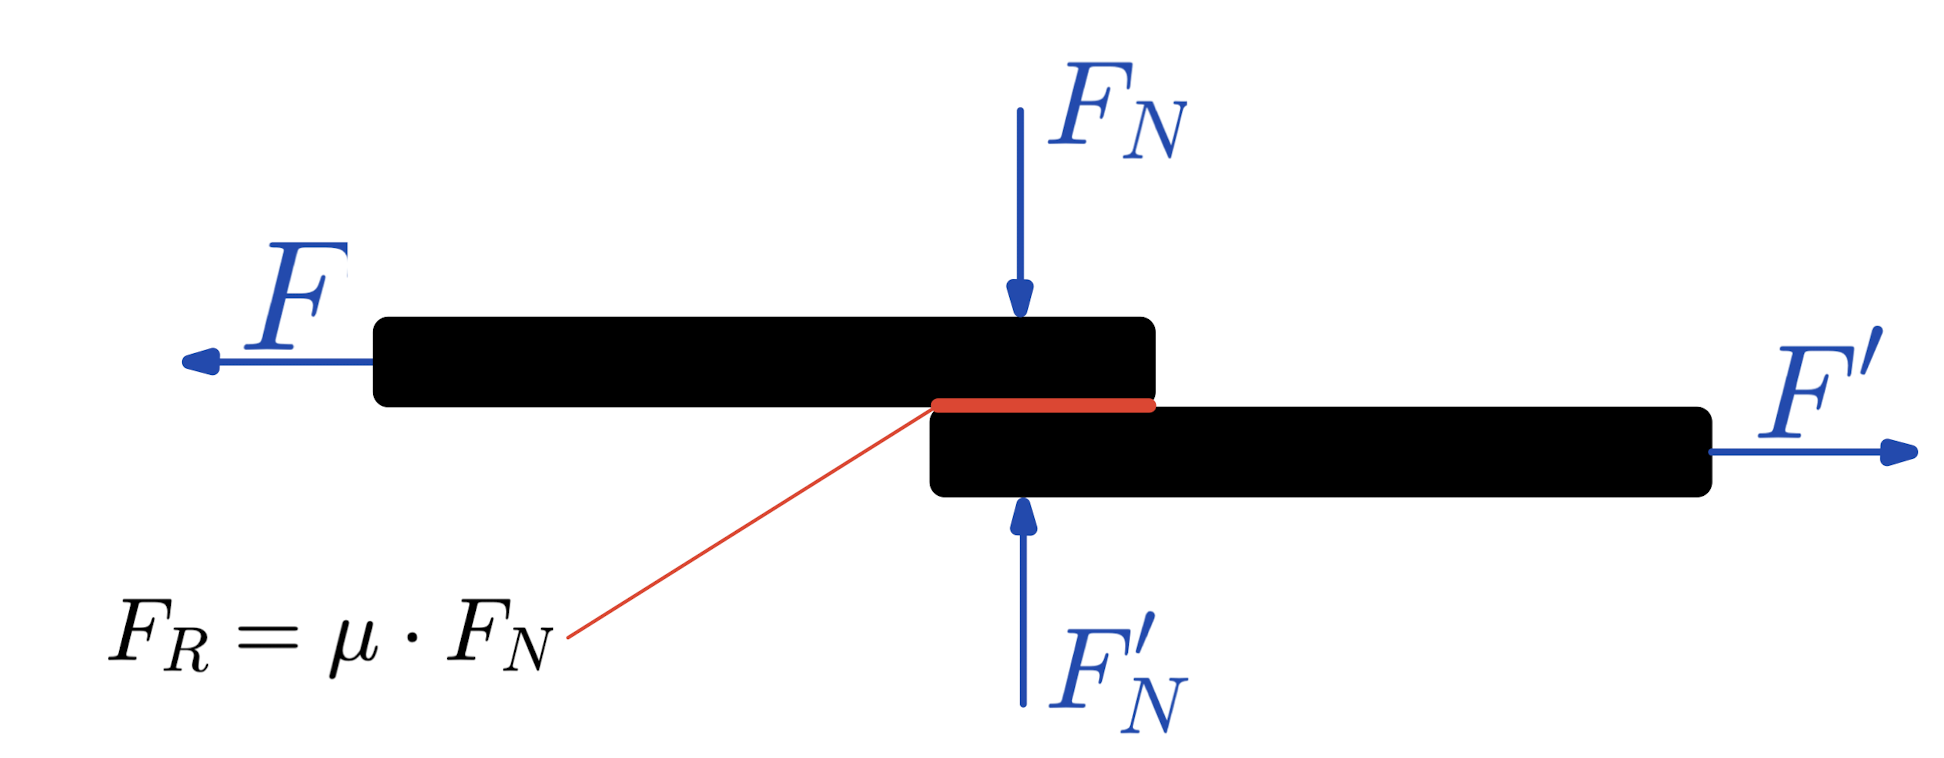
\includegraphics[width =0.6\linewidth]{MAEIP_Reibschluss}
    \end{center}
\end{footnotesize}
\subsubsection{Reibkraft \hfill ME}
    \begin{minipage}{0.6\linewidth}
        \begin{footnotesize}
            \begin{center}
                \begin{empheq}[box=\fbox]{align*}
                    F_{\text{res}} &= \sqrt{F_t^2 + F_a^2}
                    \\ F_t &= \frac{2\cdot M_2}{d}
                    \\ F_r &= F_{\text{res}} \cdot S_R = F_N \cdot \mu_H
                    \\ &= p \cdot A \cdot \mu_H = p(\pi d l) \cdot \mu_H
                    \\ A &= \pi \cdot l_{tr} \cdot d
                    \end{empheq}
            \end{center}
        \end{footnotesize}
    \end{minipage}
    \begin{minipage}{0.38\linewidth}
        \begin{scriptsize}
            \begin{center}
                \begin{align*}
                    S_R &= \text{Sicherheitsfaktor} \\ & \text{gegen Rutschen}
                    \\F_a &= \text{axiale Kräfte}
                    \\ A &= \text{Fläche}
                    \\ \mu_H &= \text{Haftreibung}
                    \\ F_t &= \text{Tangential/Umfangskraft}
                    \\(\text{greift} &\text{ direkt an Welle an})
                \end{align*}
            \end{center}
        \end{scriptsize}
    \end{minipage}

\subsubsection{Fugenpressung \hfill ME}
\begin{footnotesize}
    \begin{minipage}{0.6\linewidth}
        \begin{center}
            \begin{empheq}[box=\fbox]{align*}
                p_{\text{min}} &= \frac{F_{\text{res}}}{\mu_H \cdot \pi \cdot d \cdot l_{\text{tr}}}
                = \frac{F_{\text{res}}}{\mu_H \cdot A}
                \\p_{\text{max}} &\Rightarrow \sigma_V < \sigma_{\text{zul}}
            \end{empheq}
        \end{center}
    \end{minipage}
    \begin{minipage}{0.38\linewidth}
        \begin{center}
            \begin{align*}
                \scriptstyle p = \text{Fugendruck}\\
            \end{align*}
        \end{center}
    \end{minipage}
\end{footnotesize}

\subsubsection{Übermass U\hfill ME}
\begin{footnotesize}
   \begin{minipage}{0.6\linewidth}
       \begin{center}
           \begin{empheq}[box=\fbox]{align*}
              G &= 0.8 \cdot (R_{Wa} + R_{Ni}) 
              \\U &= U_{\text{theo}} + G
              \\U_{\text{theo}} &= d_{Wa} - d_{Ni}
              \\U_{\text{max}} &= d_{Wa, \text{max}} - d_{Ni, \text{min}}
              \\U_{\text{min}} &= d_{Wa, \text{min}} - d_{Ni, \text{max}}
           \end{empheq}
       \end{center}
   \end{minipage}
   \begin{minipage}{0.38\linewidth}
       \begin{center}
           \begin{scriptsize}
           \begin{align*}
               G &= \text{Glättung}
               \\U &= \text{Übermass}
           \end{align*}
        \end{scriptsize}
       \end{center}
   \end{minipage}
\end{footnotesize}

\subsubsection{Sicherheit gegen Rutschen \hfill ME}
\begin{footnotesize}
        \begin{center}
            \begin{empheq}[box=\fbox]{align*}
                S_R &= \frac{R}{B} = \frac{M_{t, \text{max}}}{M_t}
                \\M_{t, \text{max}} &= \frac{1}{2} \cdot d \cdot F_{t, \text{max}} = \frac{1}{2} \cdot d \cdot \mu \cdot F_{\text{Fuge}}
                \\ &= \frac{1}{2} \cdot d \cdot \mu \cdot p_{\text{Passung}} \cdot A = \frac{1}{2} \cdot d \cdot \mu \cdot p_{\text{Passung}} \cdot \pi \cdot l \cdot d
            \end{empheq}
        \end{center}
\end{footnotesize}


\subsubsection{Kegelpressverband \hfill ME}
\begin{footnotesize}
    \begin{minipage}{0.3\linewidth}
        \begin{center}
            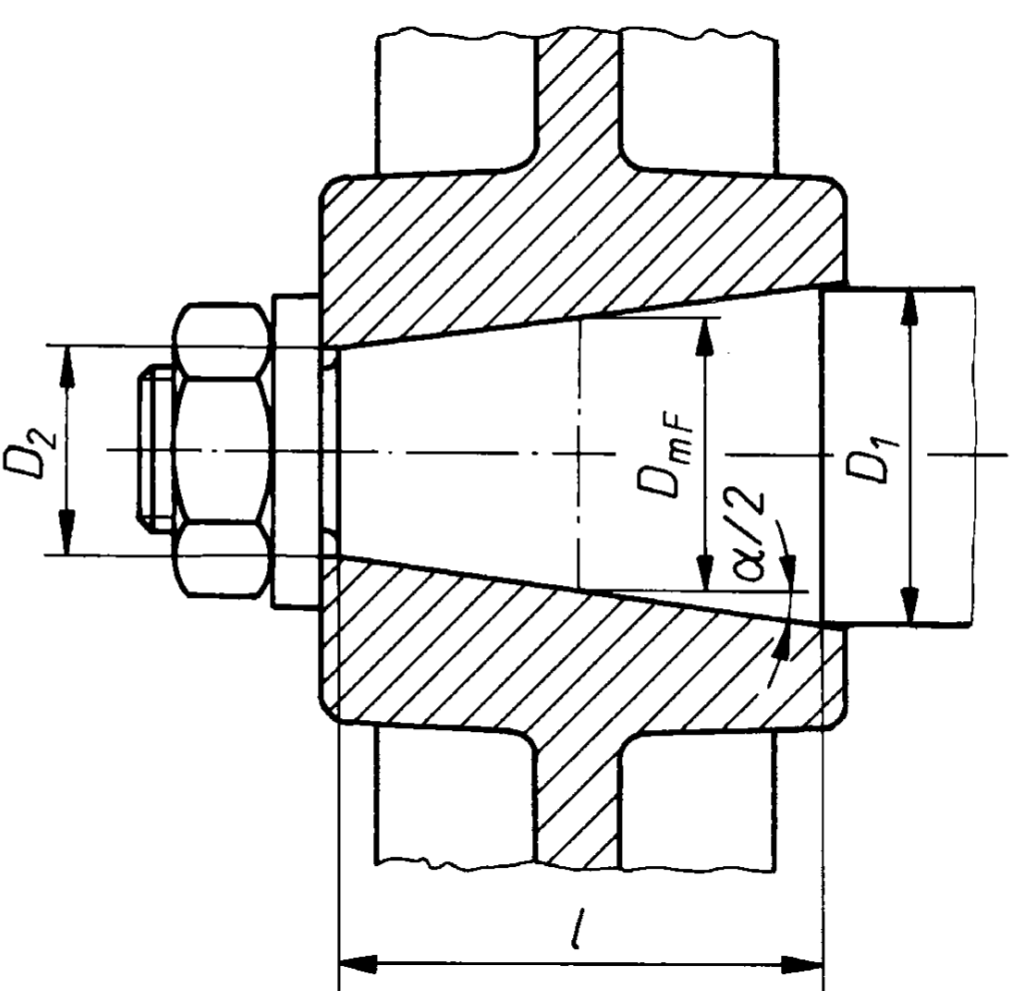
\includegraphics[width = 1.0\linewidth]{MAEIP_Kegelpressverband}
        \end{center}
    \end{minipage}
    \begin{minipage}{0.58\linewidth}
        \begin{center}
            \mathbox{
                p \leq 2 \cdot (\frac{\alpha }{2}) \cdot \frac{M_t}{\mu \cdot \pi \cdot d_m^2 \cdot l}
            }
            \scriptsize{$d_m$ = mittlerer Durchmesser} 
            \mathbox{
                U = U_{\text{theo}} + 0.8(R_{ZW} + R_{ZN})
            }
            \vspace{-1mm}
            \mathbox{
                \Delta l = \frac{U}{2 \cdot tan(\alpha)}
            }
        \end{center}
    \end{minipage}
\end{footnotesize}